\title{Lecture 8\\Representation of Structures and Semantic Neighborhoods in a Knowledge Base}

\begin{frame}
	\titlepage
\end{frame}

\begin{frame}{\\Lecture outline}
	\topline
	\RaggedRight
	A structure as a knowledge base fragment. Types of structures and roles of their elements. Relations on structures. Representation of metainformation constructions in a knowledge base. Semantic neighborhoods and their types.
\end{frame}

\begin{frame}{A structure as a knowledge base fragment}
	\topline
	\RaggedRight
	As large amounts of information accumulate in a knowledge base, it becomes necessary to identify \textbf{entire fragments} of the knowledge base and specify them by treating them \textbf{as separate entities}.

Such a knowledge base fragment is called a structure (an sc-structure).

A \textbf{\textit{structure}} is understood as a \textbf{set of
sc-elements} such that removing one of them may violate the integrity of the set.

A structure can be depicted by explicitly showing all membership pairs connecting its elements to it, or by a contour enclosing all its elements.
\end{frame}

\begin{frame}{Example of a structure represented\\as a knowledge base fragment}
	\topline
	\RaggedRight
	\begin{figure}[H]
		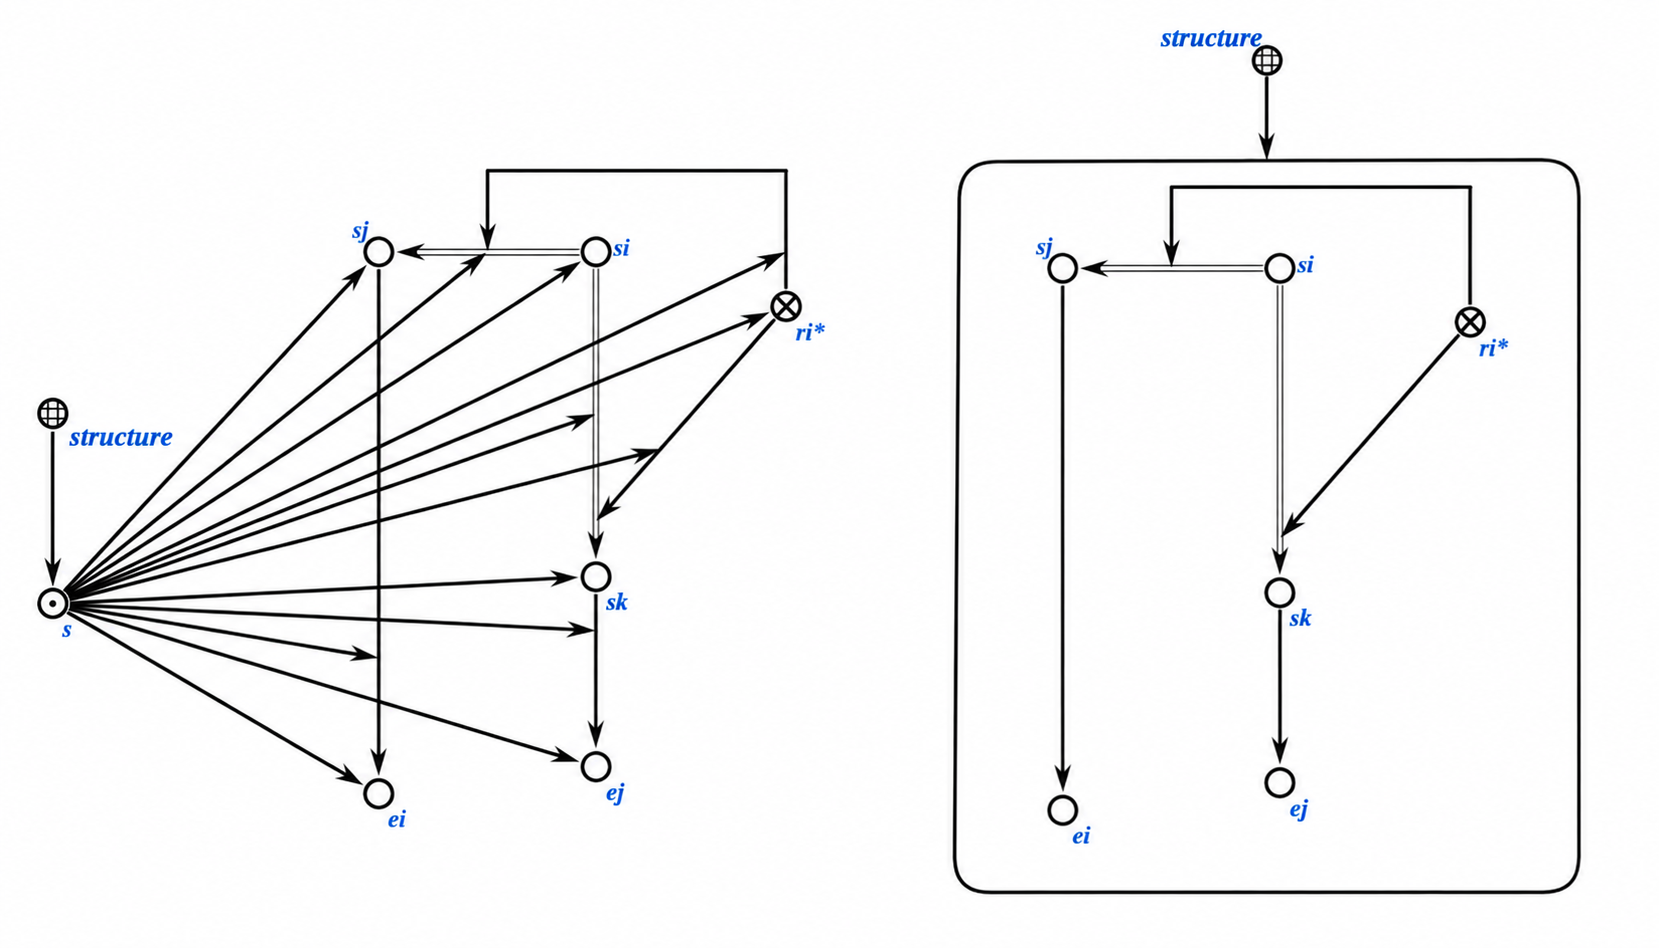
\includegraphics[height=174.24bp,keepaspectratio]{./figures/sd_structures/structure_en.png}
	\end{figure}
\end{frame}

\begin{frame}{\\Types of structures}
	\topline
	\RaggedRight
	\begin{SCn}
	\scnheader{structure}
	\begin{scnrelfromset}{partition}
		\scnitem{connected structure}
		\scnitem{disconnected structure}
	\end{scnrelfromset}
	\begin{scnrelfromset}{partition}
		\scnitem{trivial structure}
		\begin{scnindent}
			\scnidtf{structure containing no tuples}
		\end{scnindent}
		\scnitem{nontrivial structure}
		\begin{scnindent}
			\scnidtf{structure containing at least one tuple}
		\end{scnindent}
	\end{scnrelfromset}
	\end{SCn}
\end{frame}


\begin{frame}{\\Types of structures}
	\topline
	\RaggedRight
	Associate a structure represented in SC-code with a directed graph whose vertices are sc-elements and whose arcs are incidence-relation tuples connecting sc-connectors to their incident sc-elements, which are the components of those connectors. If the resulting directed graph is connected, the original structure is considered connected.

If that graph is disconnected, the original structure is considered disconnected.
\end{frame}


\begin{frame}{\\Types of structures}
	\topline
	\RaggedRight
	\vspace{10mm}

	According to stationarity, structures are divided into dynamic structures (processes), whose composition changes over time, and static structures, whose composition does not change over time.

	\begin{SCn}
	\scnheader{structure}
	\begin{scnrelfromset}{partition}
		\scnitem{process}
		\begin{scnindent}
			\scnidtf{dynamic structure}
			\scnidtf{nonstationary structure}
		\end{scnindent}
		\scnitem{static structure}
		\begin{scnindent}
			\scnidtf{stationary structure}
			\scnidtf{structure that does not change over time}
		\end{scnindent}
	\end{scnrelfromset}
	\end{SCn}
\end{frame}

\begin{frame}{\\Types of structures}
	\topline
	\RaggedRight

	According to their lifetime, structures are divided into temporary structures and permanently existing structures.

	\begin{SCn}
	\scnheader{structure}
	\begin{scnrelfromset}{partition}
		\scnitem{temporary structure}
		\scnitem{permanently existing structure}
	\end{scnrelfromset}
	\end{SCn}
\end{frame}

\begin{frame}{\\Roles of structure elements}
	\topline
	\RaggedRight
	\vspace{10mm}

	Formal representation of structures uses concepts describing the roles of elements within a structure. \textbf{\textit{structure element\scnrolesign}} is a non-basic concept, a role relation identifying all elements of each structure.

	\begin{SCn}
	\scnheader{structure element\scnrolesign}
	\begin{scnrelfromset}{partition}
		\scnitem{unrepresented set\scnrolesign}
		\scnitem{fully represented set\scnrolesign}
		\scnitem{partially represented set\scnrolesign}
		\scnitem{structure element that is not a set\scnrolesign}
	\end{scnrelfromset}
	\end{SCn}
\end{frame}

\begin{frame}{\\Roles of structure elements}
	\topline
	\RaggedRight
	\vspace{10mm}

	\begin{SCn}
	\scnheader{structure element\scnrolesign}
	\begin{scnrelfromset}{partition}
		\scnitem{maximal set\scnrolesign}
		\begin{scnindent}
			\scntext{explanation}{\RaggedRight A role relation connecting a structure to the sign of a set for which no superset exists whose sign is also an element of the same structure}
		\end{scnindent}
		\scnitem{non-maximal set\scnrolesign}
		\begin{scnindent}
			\scntext{explanation}{\RaggedRight A role relation connecting a structure to the sign of a set for which a superset exists within that structure.}
		\end{scnindent}
	\end{scnrelfromset}
	\end{SCn}
\end{frame}

\begin{frame}{\\Roles of structure elements}
	\topline
	\RaggedRight
	\vspace{5mm}

	\begin{SCn}
	\small
	\scnheader{structure element\scnrolesign}
	\begin{scnrelfromset}{partition}
		\scnitem{primary element\scnrolesign}
		\begin{scnindent}
			\scntext{explanation}{\RaggedRight A role relation identifying an (atomic) structure element with no elements belonging to it. The corresponding membership pair may exist but lie outside this structure.}
		\end{scnindent}
		\scnitem{secondary element\scnrolesign}
		\begin{scnindent}
			\scnidtf{element of this structure with a semantic level greater than 2\scnrolesign}
			\scnidtf{non-primary element\scnrolesign}
			\scntext{explanation}{\RaggedRight A role relation identifying a structure element that denotes a set of elements, at least one of which must belong to the structure.}
		\end{scnindent}
	\end{scnrelfromset}
	\end{SCn}
\end{frame}

\begin{frame}{\\Roles of structure elements}
	\topline
	\RaggedRight

	\scnheader{structure element\scnrolesign}
	\begin{scnrelfromset}{partition}
		\scnitem{first-level structure\scnrolesign}
		\begin{scnindent}
			\scntext{explanation}{\RaggedRight tuple of primary elements, trivial structure of primary elements, or class of primary elements}
		\end{scnindent}
		\scnitem{secondary structure\scnrolesign}
		\begin{scnindent}
			\scntext{explanation}{\RaggedRight structure with at least one secondary element\scnrolesign}
		\end{scnindent}
	\end{scnrelfromset}
\end{frame}

\begin{frame}{\\Example of structure element roles}
	\topline
	\RaggedRight
	\begin{figure}[H]
		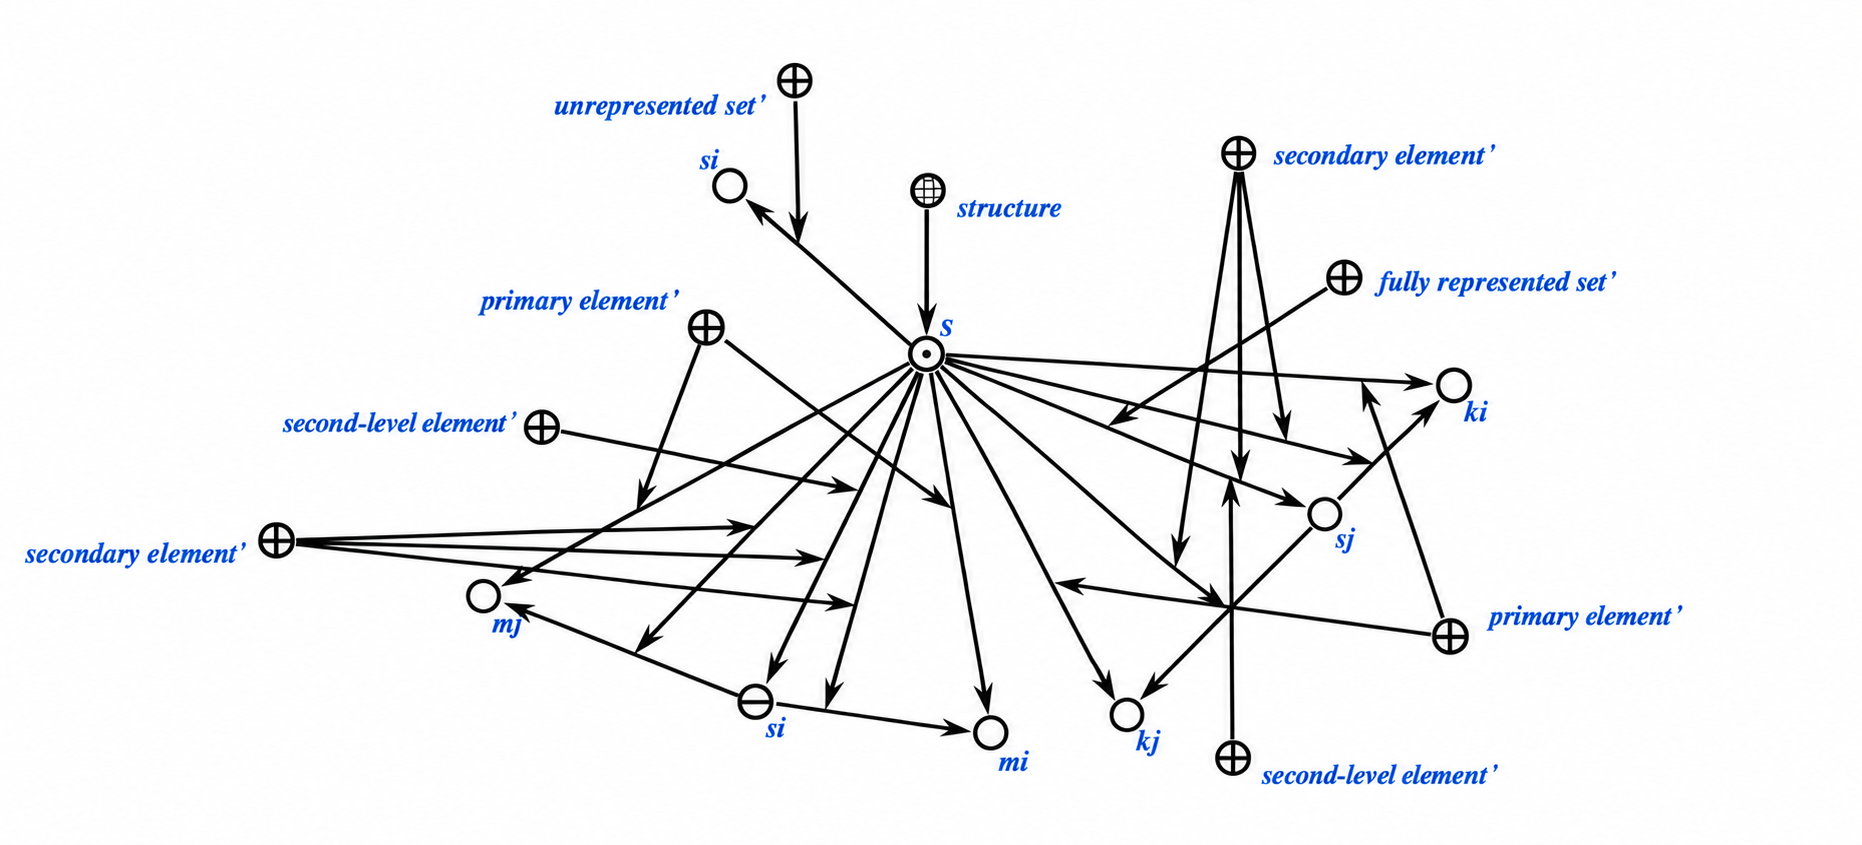
\includegraphics[width=0.94\linewidth,height=0.72\textheight,keepaspectratio]{./figures/sd_structures/roles_en.png}
	\end{figure}
\end{frame}

\begin{frame}{\\Relations on structures}
	\topline
	\RaggedRight
	\scnheader{binary relation*}
	\scnhaselement{polymorphism relation* }
		\begin{scnindent}
			\scnsubset{correspondence*}
		\end{scnindent}
	\scnhaselement{polymorphism*}
	\scnhaselement{homomorphism relation*}
		\begin{scnindent}
		\scnsubset{correspondence*}
		\end{scnindent}
	\scnhaselement{homomorphism*}
	\scnhaselement{isomorphism relation*}
		\begin{scnindent}
		\scnsubset{correspondence*}
		\end{scnindent}
	\scnhaselement{isomorphism*}
	\scnhaselement{automorphism relation*}
		\begin{scnindent}
		\scnsubset{correspondence*}
		\end{scnindent}
	\scnhaselement{automorphism*}
\end{frame}

\begin{frame}{\\Relations on structures}
	\topline
	\RaggedRight

	\scnheader{polymorphism relation* }
	\scntext{explanation}{\RaggedRight polymorphism relation* is a correspondence between structures in which each domain element (in the first structure) is associated with one or more codomain elements (in the second structure), and at least one domain element is associated with two or more codomain elements.}
\end{frame}

\begin{frame}{\\Relations on structures}
	\topline
	\RaggedRight

	\scnheader{homomorphism relation*}
	\scntext{explanation}{\RaggedRight homomorphism relation* is a correspondence between structures in which each domain element (in the first structure) is associated with exactly one codomain element (in the second structure).}
\end{frame}

\begin{frame}{\\Relations on structures}
	\topline
	\RaggedRight

	\scnheader{isomorphism relation*}
	\scntext{explanation}{\RaggedRight isomorphism relation* is a homomorphism relation* in which every codomain element has exactly one corresponding domain element.}


	\scnheader{automorphism relation*}
	\scntext{explanation}{\RaggedRight automorphism relation* is an isomorphism relation* whose domain and codomain coincide.}
\end{frame}

\begin{frame}{\\Relations on structures}
	\topline
	\RaggedRight

	\scnheader{structural analogy*}
	\scnsubset{correspondence*}
	\scniselement{binary relation*}
	\scntext{explanation}{\RaggedRight structural analogy* is a correspondence* between structures recording an analogy between their substructures (subsets). Each ordered pair belonging to structural analogy* can be associated with a set of pairs specifying similarities* between some substructures and differences* between others.}
\end{frame}

\begin{frame}{\\Example}
	\topline
	\RaggedRight

	\begin{figure}[b]
		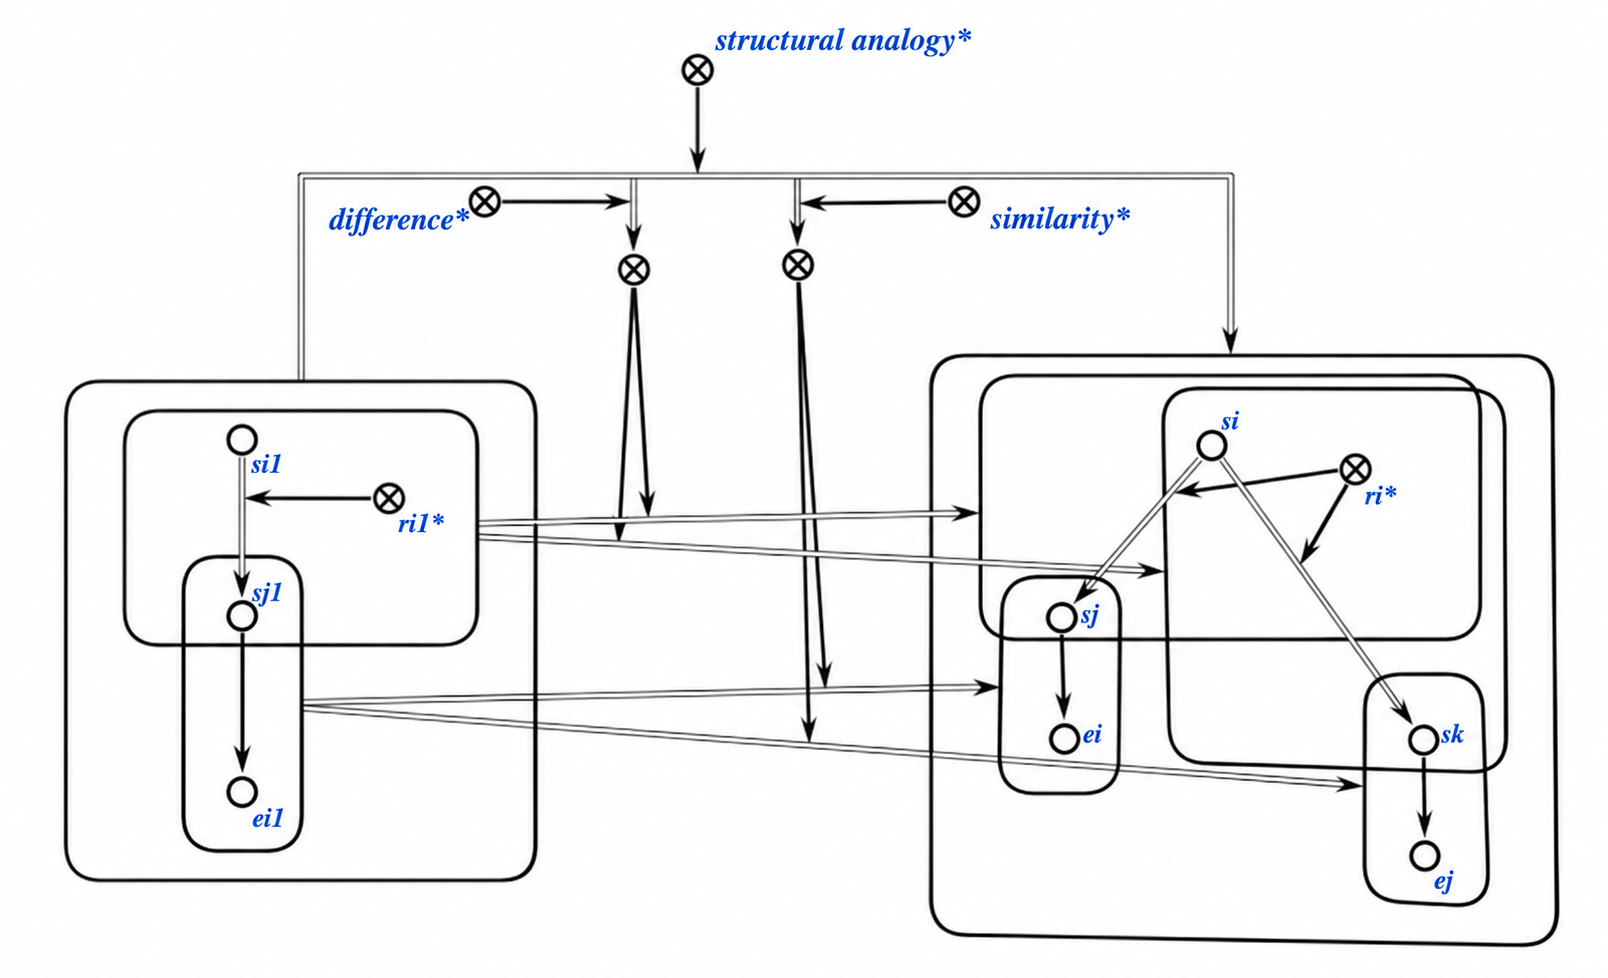
\includegraphics[height=161.4bp,keepaspectratio]{./figures/sd_structures/analog_en.png}
	\end{figure}
\end{frame}

\begin{frame}{\\Generalized structure}
	\topline
	\RaggedRight
	\vspace{10mm}
	\begin{figure}[b]
		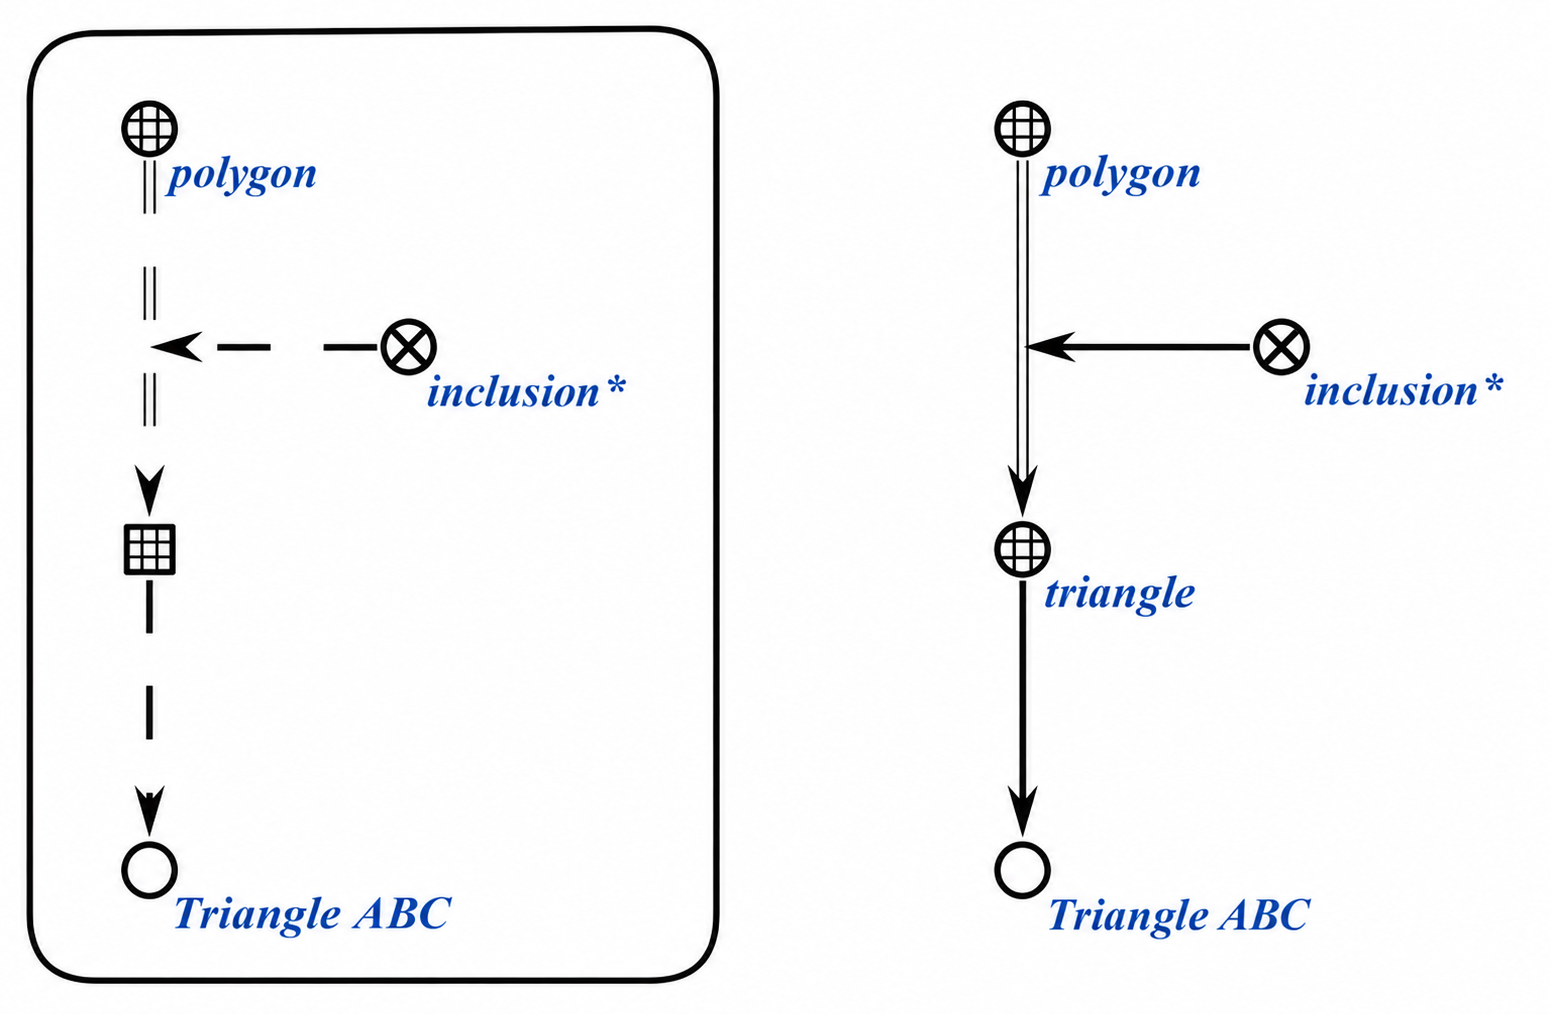
\includegraphics[height=198bp,keepaspectratio]{./figures/sd_structures/generalized_structure_en.png}
	\end{figure}
\end{frame}

\begin{frame}{\\The concept of a semantic neighborhood}
	\topline
	\RaggedRight

	\vspace{5mm}
	To specify individual entities in a knowledge base, we introduce the concept of a \textit{\textbf{semantic neighborhood}}.

A semantic neighborhood is a specification of a given entity whose sign is identified as the key element of the specification. Unlike other types of knowledge, a semantic neighborhood has only one key element.

Entities can be specified using different sets of features. The same entity may also need to be specified from different perspectives, with those perspectives explicitly recorded in the knowledge base.

For example, a person can be described from professional, medical, civic and other perspectives.
\end{frame}

\begin{frame}{\\Example}
	\topline
	\RaggedRight
	\vspace{10mm}

	\begin{figure}[H]
		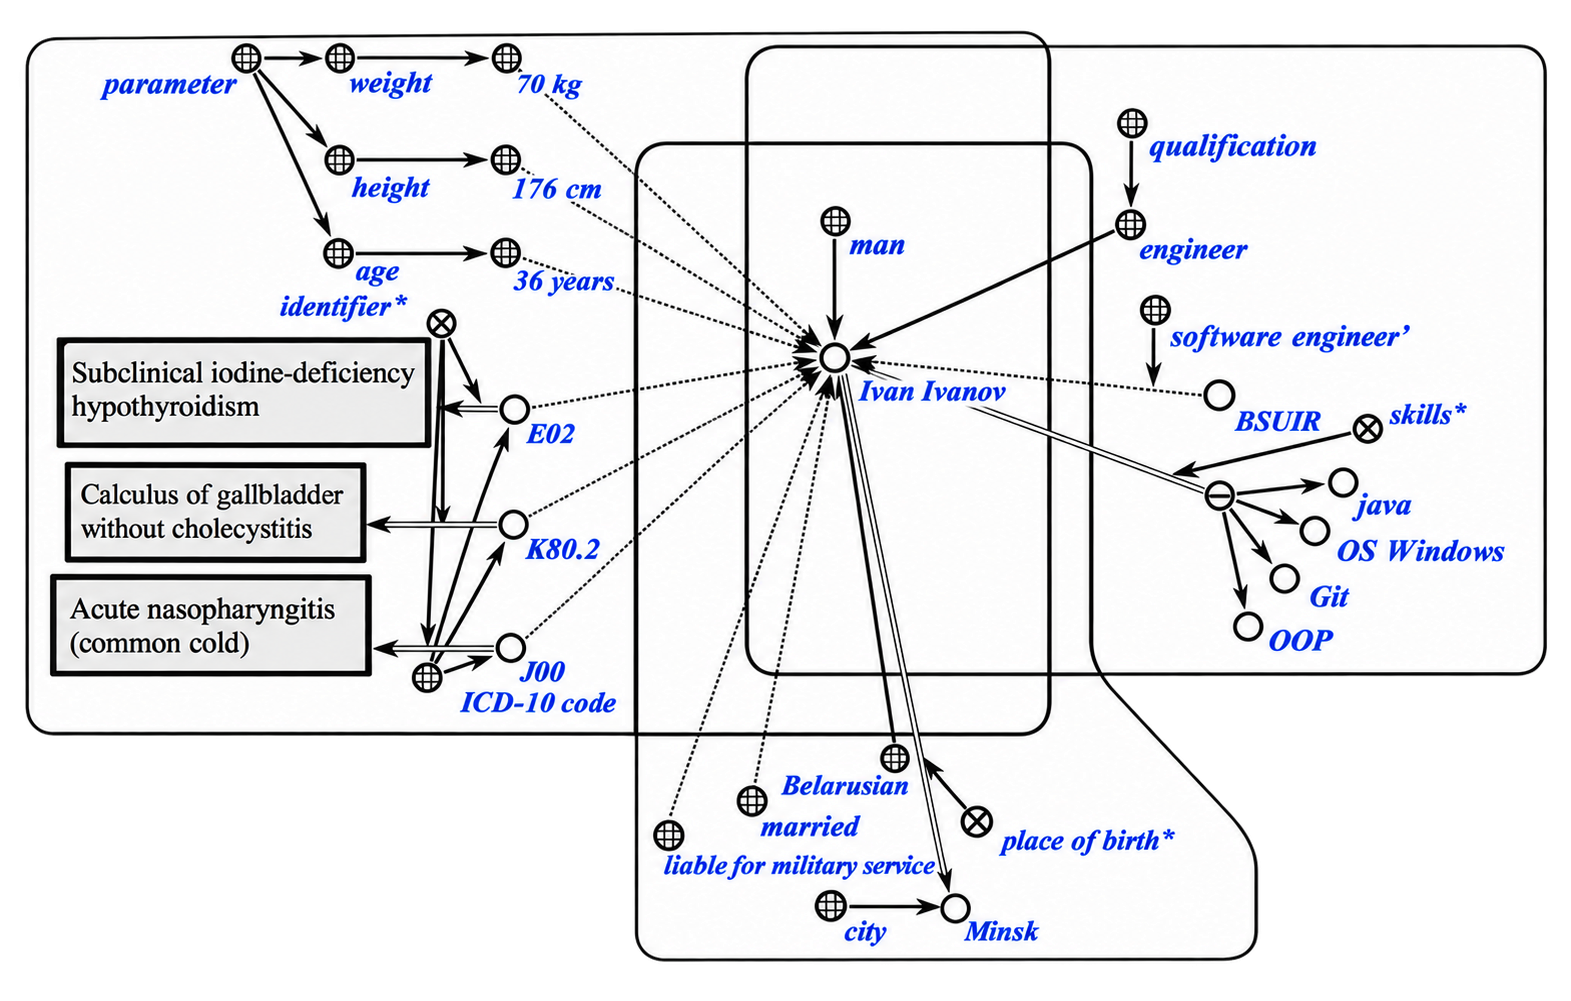
\includegraphics[height=194.7bp,keepaspectratio]{./figures/sd_structures/example_en.png}
	\end{figure}
\end{frame}

\begin{frame}{\\The concept of a semantic neighborhood}
	\topline
	\RaggedRight

	\begin{SCn}
	\scnheader{semantic neighborhood}
	\scnidtf{description of a given entity whose sign is identified as the key element of the specification}
	\scnsubset{knowledge}
	\scnsuperset{semantic neighborhood of incident connectors}
	\scnsuperset{complete semantic neighborhood}
	\scnsuperset{basic semantic neighborhood}
	\scnsuperset{specialized semantic neighborhood}
	\end{SCn}

\end{frame}

\begin{frame}{\\Types of semantic neighborhoods}
	\topline
	\RaggedRight

	\begin{SCn}
	\scnheader{semantic neighborhood of incident connectors}
	\scnsuperset{semantic neighborhood of outgoing arcs}
	\scnsuperset{semantic neighborhood of incoming arcs}
	\scntext{explanation}{\RaggedRight a type of semantic neighborhood containing all connectors incident to a given element and all elements incident to those connectors}
	\end{SCn}

\end{frame}

\begin{frame}{\\Types of semantic neighborhoods}
	\topline
	\RaggedRight

	\begin{SCn}
	\scnheader{complete semantic neighborhood}
	\scnidtf{complete specification of an entity being described}

	\scnheader{basic semantic neighborhood}
	\scnidtf{minimally sufficient semantic neighborhood}

	\scnheader{specialized semantic neighborhood}
	\scnidtf{a type of semantic neighborhood whose set of connections is specified separately for each neighborhood type}
	\end{SCn}

\end{frame}

\begin{frame}{\\Types of semantic neighborhoods}
	\topline
	\RaggedRight

	\begin{SCn}
	\scnheader{specialized semantic neighborhood}
	\scnsuperset{explanation}
	\scnsuperset{note}
	\scnsuperset{instance identification rule}
	\scnsuperset{terminological semantic neighborhood}
	\scnsuperset{set-theoretic semantic neighborhood}
	\scnsuperset{logical semantic neighborhood}
	\scnsuperset{description of a typical instance}
	\scnsuperset{description of a decomposition}
	\end{SCn}

\end{frame}
